\documentclass[tikz,border=0pt]{standalone}
\usepackage{amsmath,newpxtext,newpxmath}
\begin{document}
% Created by tikzDevice version 0.12.6 on 2026-11-21 20:58:43
% !TEX encoding = UTF-8 Unicode
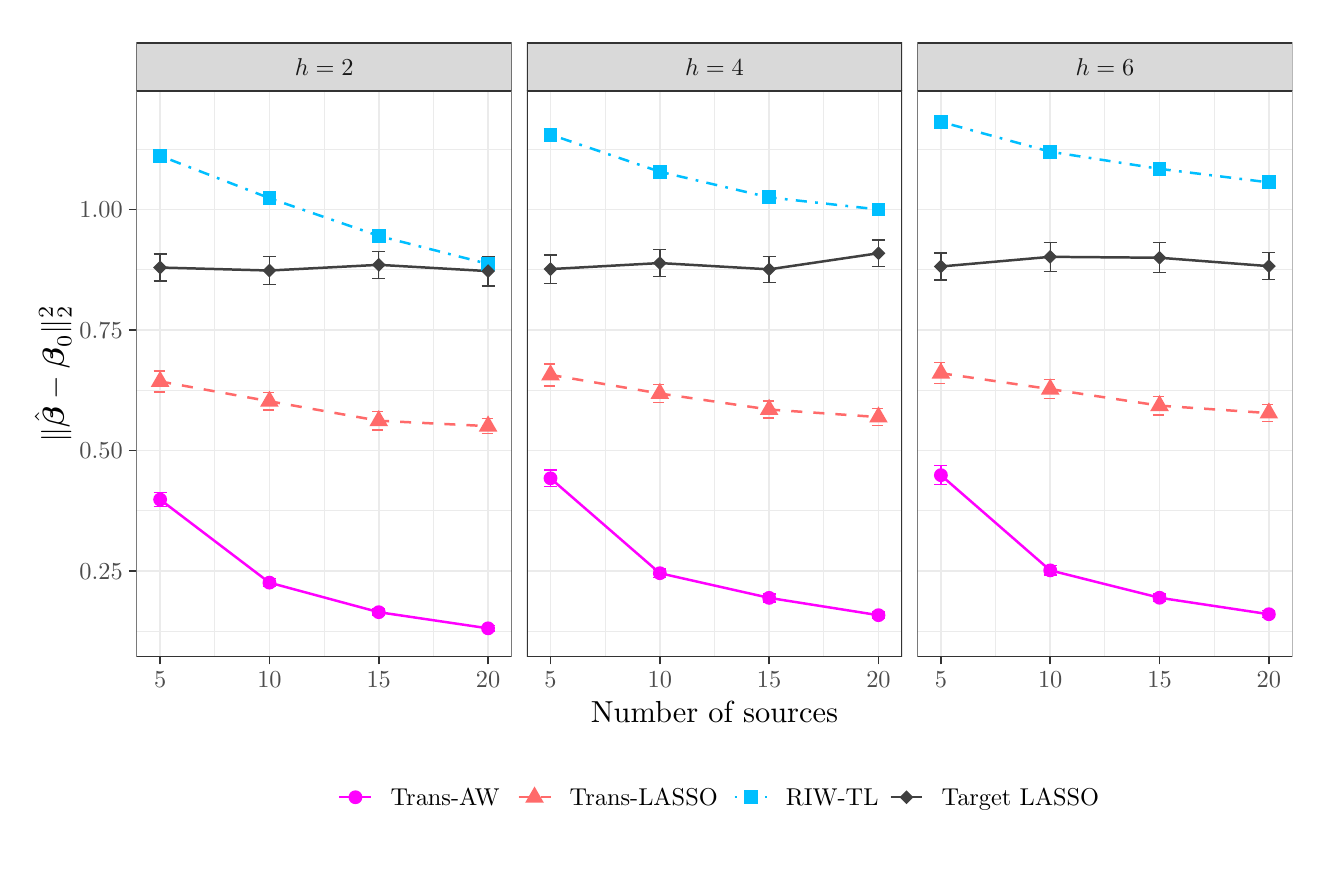
\begin{tikzpicture}[x=1pt,y=1pt]
\definecolor{fillColor}{RGB}{255,255,255}
\path[use as bounding box,fill=fillColor,fill opacity=0.00] (0,0) rectangle (462.53,296.31);
\begin{scope}
\path[clip] (  0.00,  0.00) rectangle (462.53,296.31);
\definecolor{drawColor}{RGB}{255,255,255}
\definecolor{fillColor}{RGB}{255,255,255}

\path[draw=drawColor,line width= 0.6pt,line join=round,line cap=round,fill=fillColor] (  0.00,  0.00) rectangle (462.53,296.31);
\end{scope}
\begin{scope}
\path[clip] ( 39.32, 68.96) rectangle (174.89,273.43);
\definecolor{fillColor}{RGB}{255,255,255}

\path[fill=fillColor] ( 39.32, 68.96) rectangle (174.89,273.43);
\definecolor{drawColor}{gray}{0.92}

\path[draw=drawColor,line width= 0.3pt,line join=round] ( 39.32, 78.21) --
	(174.89, 78.21);

\path[draw=drawColor,line width= 0.3pt,line join=round] ( 39.32,121.77) --
	(174.89,121.77);

\path[draw=drawColor,line width= 0.3pt,line join=round] ( 39.32,165.33) --
	(174.89,165.33);

\path[draw=drawColor,line width= 0.3pt,line join=round] ( 39.32,208.88) --
	(174.89,208.88);

\path[draw=drawColor,line width= 0.3pt,line join=round] ( 39.32,252.44) --
	(174.89,252.44);

\path[draw=drawColor,line width= 0.3pt,line join=round] ( 67.61, 68.96) --
	( 67.61,273.43);

\path[draw=drawColor,line width= 0.3pt,line join=round] (107.11, 68.96) --
	(107.11,273.43);

\path[draw=drawColor,line width= 0.3pt,line join=round] (146.61, 68.96) --
	(146.61,273.43);

\path[draw=drawColor,line width= 0.6pt,line join=round] ( 39.32, 99.99) --
	(174.89, 99.99);

\path[draw=drawColor,line width= 0.6pt,line join=round] ( 39.32,143.55) --
	(174.89,143.55);

\path[draw=drawColor,line width= 0.6pt,line join=round] ( 39.32,187.10) --
	(174.89,187.10);

\path[draw=drawColor,line width= 0.6pt,line join=round] ( 39.32,230.66) --
	(174.89,230.66);

\path[draw=drawColor,line width= 0.6pt,line join=round] ( 47.86, 68.96) --
	( 47.86,273.43);

\path[draw=drawColor,line width= 0.6pt,line join=round] ( 87.36, 68.96) --
	( 87.36,273.43);

\path[draw=drawColor,line width= 0.6pt,line join=round] (126.86, 68.96) --
	(126.86,273.43);

\path[draw=drawColor,line width= 0.6pt,line join=round] (166.36, 68.96) --
	(166.36,273.43);
\definecolor{drawColor}{RGB}{0,191,255}

\path[draw=drawColor,line width= 0.5pt,dash pattern=on 1pt off 3pt on 4pt off 3pt ,line join=round] ( 45.49,251.97) --
	( 50.23,251.97);

\path[draw=drawColor,line width= 0.5pt,dash pattern=on 1pt off 3pt on 4pt off 3pt ,line join=round] ( 47.86,251.97) --
	( 47.86,248.05);

\path[draw=drawColor,line width= 0.5pt,dash pattern=on 1pt off 3pt on 4pt off 3pt ,line join=round] ( 45.49,248.05) --
	( 50.23,248.05);

\path[draw=drawColor,line width= 0.5pt,dash pattern=on 1pt off 3pt on 4pt off 3pt ,line join=round] ( 84.99,236.49) --
	( 89.73,236.49);

\path[draw=drawColor,line width= 0.5pt,dash pattern=on 1pt off 3pt on 4pt off 3pt ,line join=round] ( 87.36,236.49) --
	( 87.36,232.90);

\path[draw=drawColor,line width= 0.5pt,dash pattern=on 1pt off 3pt on 4pt off 3pt ,line join=round] ( 84.99,232.90) --
	( 89.73,232.90);

\path[draw=drawColor,line width= 0.5pt,dash pattern=on 1pt off 3pt on 4pt off 3pt ,line join=round] (124.49,222.71) --
	(129.23,222.71);

\path[draw=drawColor,line width= 0.5pt,dash pattern=on 1pt off 3pt on 4pt off 3pt ,line join=round] (126.86,222.71) --
	(126.86,219.41);

\path[draw=drawColor,line width= 0.5pt,dash pattern=on 1pt off 3pt on 4pt off 3pt ,line join=round] (124.49,219.41) --
	(129.23,219.41);

\path[draw=drawColor,line width= 0.5pt,dash pattern=on 1pt off 3pt on 4pt off 3pt ,line join=round] (163.99,212.36) --
	(168.73,212.36);

\path[draw=drawColor,line width= 0.5pt,dash pattern=on 1pt off 3pt on 4pt off 3pt ,line join=round] (166.36,212.36) --
	(166.36,209.53);

\path[draw=drawColor,line width= 0.5pt,dash pattern=on 1pt off 3pt on 4pt off 3pt ,line join=round] (163.99,209.53) --
	(168.73,209.53);
\definecolor{drawColor}{gray}{0.25}

\path[draw=drawColor,line width= 0.5pt,line join=round] ( 45.49,214.53) --
	( 50.23,214.53);

\path[draw=drawColor,line width= 0.5pt,line join=round] ( 47.86,214.53) --
	( 47.86,204.75);

\path[draw=drawColor,line width= 0.5pt,line join=round] ( 45.49,204.75) --
	( 50.23,204.75);

\path[draw=drawColor,line width= 0.5pt,line join=round] ( 84.99,213.63) --
	( 89.73,213.63);

\path[draw=drawColor,line width= 0.5pt,line join=round] ( 87.36,213.63) --
	( 87.36,203.47);

\path[draw=drawColor,line width= 0.5pt,line join=round] ( 84.99,203.47) --
	( 89.73,203.47);

\path[draw=drawColor,line width= 0.5pt,line join=round] (124.49,215.53) --
	(129.23,215.53);

\path[draw=drawColor,line width= 0.5pt,line join=round] (126.86,215.53) --
	(126.86,205.68);

\path[draw=drawColor,line width= 0.5pt,line join=round] (124.49,205.68) --
	(129.23,205.68);

\path[draw=drawColor,line width= 0.5pt,line join=round] (163.99,213.68) --
	(168.73,213.68);

\path[draw=drawColor,line width= 0.5pt,line join=round] (166.36,213.68) --
	(166.36,203.01);

\path[draw=drawColor,line width= 0.5pt,line join=round] (163.99,203.01) --
	(168.73,203.01);
\definecolor{drawColor}{RGB}{255,0,255}

\path[draw=drawColor,line width= 0.5pt,line join=round] ( 45.49,128.36) --
	( 50.23,128.36);

\path[draw=drawColor,line width= 0.5pt,line join=round] ( 47.86,128.36) --
	( 47.86,123.23);

\path[draw=drawColor,line width= 0.5pt,line join=round] ( 45.49,123.23) --
	( 50.23,123.23);

\path[draw=drawColor,line width= 0.5pt,line join=round] ( 84.99, 97.18) --
	( 89.73, 97.18);

\path[draw=drawColor,line width= 0.5pt,line join=round] ( 87.36, 97.18) --
	( 87.36, 94.36);

\path[draw=drawColor,line width= 0.5pt,line join=round] ( 84.99, 94.36) --
	( 89.73, 94.36);

\path[draw=drawColor,line width= 0.5pt,line join=round] (124.49, 86.19) --
	(129.23, 86.19);

\path[draw=drawColor,line width= 0.5pt,line join=round] (126.86, 86.19) --
	(126.86, 84.01);

\path[draw=drawColor,line width= 0.5pt,line join=round] (124.49, 84.01) --
	(129.23, 84.01);

\path[draw=drawColor,line width= 0.5pt,line join=round] (163.99, 80.27) --
	(168.73, 80.27);

\path[draw=drawColor,line width= 0.5pt,line join=round] (166.36, 80.27) --
	(166.36, 78.25);

\path[draw=drawColor,line width= 0.5pt,line join=round] (163.99, 78.25) --
	(168.73, 78.25);
\definecolor{drawColor}{RGB}{255,106,106}

\path[draw=drawColor,line width= 0.5pt,dash pattern=on 4pt off 4pt ,line join=round] ( 45.49,172.23) --
	( 50.23,172.23);

\path[draw=drawColor,line width= 0.5pt,dash pattern=on 4pt off 4pt ,line join=round] ( 47.86,172.23) --
	( 47.86,164.71);

\path[draw=drawColor,line width= 0.5pt,dash pattern=on 4pt off 4pt ,line join=round] ( 45.49,164.71) --
	( 50.23,164.71);

\path[draw=drawColor,line width= 0.5pt,dash pattern=on 4pt off 4pt ,line join=round] ( 84.99,164.49) --
	( 89.73,164.49);

\path[draw=drawColor,line width= 0.5pt,dash pattern=on 4pt off 4pt ,line join=round] ( 87.36,164.49) --
	( 87.36,158.13);

\path[draw=drawColor,line width= 0.5pt,dash pattern=on 4pt off 4pt ,line join=round] ( 84.99,158.13) --
	( 89.73,158.13);

\path[draw=drawColor,line width= 0.5pt,dash pattern=on 4pt off 4pt ,line join=round] (124.49,157.58) --
	(129.23,157.58);

\path[draw=drawColor,line width= 0.5pt,dash pattern=on 4pt off 4pt ,line join=round] (126.86,157.58) --
	(126.86,150.95);

\path[draw=drawColor,line width= 0.5pt,dash pattern=on 4pt off 4pt ,line join=round] (124.49,150.95) --
	(129.23,150.95);

\path[draw=drawColor,line width= 0.5pt,dash pattern=on 4pt off 4pt ,line join=round] (163.99,155.03) --
	(168.73,155.03);

\path[draw=drawColor,line width= 0.5pt,dash pattern=on 4pt off 4pt ,line join=round] (166.36,155.03) --
	(166.36,149.60);

\path[draw=drawColor,line width= 0.5pt,dash pattern=on 4pt off 4pt ,line join=round] (163.99,149.60) --
	(168.73,149.60);
\definecolor{drawColor}{RGB}{255,0,255}

\path[draw=drawColor,line width= 0.9pt,line join=round] ( 47.86,125.80) --
	( 87.36, 95.77) --
	(126.86, 85.10) --
	(166.36, 79.26);
\definecolor{drawColor}{RGB}{255,106,106}

\path[draw=drawColor,line width= 0.9pt,dash pattern=on 4pt off 4pt ,line join=round] ( 47.86,168.47) --
	( 87.36,161.31) --
	(126.86,154.27) --
	(166.36,152.32);
\definecolor{drawColor}{RGB}{0,191,255}

\path[draw=drawColor,line width= 0.9pt,dash pattern=on 1pt off 3pt on 4pt off 3pt ,line join=round] ( 47.86,250.01) --
	( 87.36,234.70) --
	(126.86,221.06) --
	(166.36,210.94);
\definecolor{drawColor}{gray}{0.25}

\path[draw=drawColor,line width= 0.9pt,line join=round] ( 47.86,209.64) --
	( 87.36,208.55) --
	(126.86,210.61) --
	(166.36,208.34);
\definecolor{fillColor}{RGB}{0,191,255}

\path[fill=fillColor] ( 45.36,247.51) --
	( 50.35,247.51) --
	( 50.35,252.51) --
	( 45.36,252.51) --
	cycle;

\path[fill=fillColor] ( 84.86,232.20) --
	( 89.86,232.20) --
	( 89.86,237.20) --
	( 84.86,237.20) --
	cycle;

\path[fill=fillColor] (124.36,218.56) --
	(129.36,218.56) --
	(129.36,223.56) --
	(124.36,223.56) --
	cycle;

\path[fill=fillColor] (163.86,208.45) --
	(168.86,208.45) --
	(168.86,213.44) --
	(163.86,213.44) --
	cycle;
\definecolor{fillColor}{gray}{0.25}

\path[fill=fillColor] ( 45.36,209.64) --
	( 47.86,212.14) --
	( 50.35,209.64) --
	( 47.86,207.14) --
	cycle;

\path[fill=fillColor] ( 84.86,208.55) --
	( 87.36,211.05) --
	( 89.86,208.55) --
	( 87.36,206.05) --
	cycle;

\path[fill=fillColor] (124.36,210.61) --
	(126.86,213.10) --
	(129.36,210.61) --
	(126.86,208.11) --
	cycle;

\path[fill=fillColor] (163.86,208.34) --
	(166.36,210.84) --
	(168.86,208.34) --
	(166.36,205.84) --
	cycle;
\definecolor{fillColor}{RGB}{255,0,255}

\path[fill=fillColor] ( 47.86,125.80) circle (  2.50);

\path[fill=fillColor] ( 87.36, 95.77) circle (  2.50);

\path[fill=fillColor] (126.86, 85.10) circle (  2.50);

\path[fill=fillColor] (166.36, 79.26) circle (  2.50);
\definecolor{fillColor}{RGB}{255,106,106}

\path[fill=fillColor] ( 47.86,172.35) --
	( 51.22,166.53) --
	( 44.49,166.53) --
	cycle;

\path[fill=fillColor] ( 87.36,165.20) --
	( 90.72,159.37) --
	( 83.99,159.37) --
	cycle;

\path[fill=fillColor] (126.86,158.15) --
	(130.22,152.33) --
	(123.50,152.33) --
	cycle;

\path[fill=fillColor] (166.36,156.20) --
	(169.72,150.37) --
	(163.00,150.37) --
	cycle;
\definecolor{drawColor}{gray}{0.20}

\path[draw=drawColor,line width= 0.6pt,line join=round,line cap=round] ( 39.32, 68.96) rectangle (174.89,273.43);
\end{scope}
\begin{scope}
\path[clip] (180.39, 68.96) rectangle (315.96,273.43);
\definecolor{fillColor}{RGB}{255,255,255}

\path[fill=fillColor] (180.39, 68.96) rectangle (315.96,273.43);
\definecolor{drawColor}{gray}{0.92}

\path[draw=drawColor,line width= 0.3pt,line join=round] (180.39, 78.21) --
	(315.96, 78.21);

\path[draw=drawColor,line width= 0.3pt,line join=round] (180.39,121.77) --
	(315.96,121.77);

\path[draw=drawColor,line width= 0.3pt,line join=round] (180.39,165.33) --
	(315.96,165.33);

\path[draw=drawColor,line width= 0.3pt,line join=round] (180.39,208.88) --
	(315.96,208.88);

\path[draw=drawColor,line width= 0.3pt,line join=round] (180.39,252.44) --
	(315.96,252.44);

\path[draw=drawColor,line width= 0.3pt,line join=round] (208.68, 68.96) --
	(208.68,273.43);

\path[draw=drawColor,line width= 0.3pt,line join=round] (248.18, 68.96) --
	(248.18,273.43);

\path[draw=drawColor,line width= 0.3pt,line join=round] (287.68, 68.96) --
	(287.68,273.43);

\path[draw=drawColor,line width= 0.6pt,line join=round] (180.39, 99.99) --
	(315.96, 99.99);

\path[draw=drawColor,line width= 0.6pt,line join=round] (180.39,143.55) --
	(315.96,143.55);

\path[draw=drawColor,line width= 0.6pt,line join=round] (180.39,187.10) --
	(315.96,187.10);

\path[draw=drawColor,line width= 0.6pt,line join=round] (180.39,230.66) --
	(315.96,230.66);

\path[draw=drawColor,line width= 0.6pt,line join=round] (188.92, 68.96) --
	(188.92,273.43);

\path[draw=drawColor,line width= 0.6pt,line join=round] (228.43, 68.96) --
	(228.43,273.43);

\path[draw=drawColor,line width= 0.6pt,line join=round] (267.93, 68.96) --
	(267.93,273.43);

\path[draw=drawColor,line width= 0.6pt,line join=round] (307.43, 68.96) --
	(307.43,273.43);
\definecolor{drawColor}{RGB}{0,191,255}

\path[draw=drawColor,line width= 0.5pt,dash pattern=on 1pt off 3pt on 4pt off 3pt ,line join=round] (186.55,259.65) --
	(191.29,259.65);

\path[draw=drawColor,line width= 0.5pt,dash pattern=on 1pt off 3pt on 4pt off 3pt ,line join=round] (188.92,259.65) --
	(188.92,255.68);

\path[draw=drawColor,line width= 0.5pt,dash pattern=on 1pt off 3pt on 4pt off 3pt ,line join=round] (186.55,255.68) --
	(191.29,255.68);

\path[draw=drawColor,line width= 0.5pt,dash pattern=on 1pt off 3pt on 4pt off 3pt ,line join=round] (226.06,245.93) --
	(230.80,245.93);

\path[draw=drawColor,line width= 0.5pt,dash pattern=on 1pt off 3pt on 4pt off 3pt ,line join=round] (228.43,245.93) --
	(228.43,242.58);

\path[draw=drawColor,line width= 0.5pt,dash pattern=on 1pt off 3pt on 4pt off 3pt ,line join=round] (226.06,242.58) --
	(230.80,242.58);

\path[draw=drawColor,line width= 0.5pt,dash pattern=on 1pt off 3pt on 4pt off 3pt ,line join=round] (265.56,236.61) --
	(270.30,236.61);

\path[draw=drawColor,line width= 0.5pt,dash pattern=on 1pt off 3pt on 4pt off 3pt ,line join=round] (267.93,236.61) --
	(267.93,233.35);

\path[draw=drawColor,line width= 0.5pt,dash pattern=on 1pt off 3pt on 4pt off 3pt ,line join=round] (265.56,233.35) --
	(270.30,233.35);

\path[draw=drawColor,line width= 0.5pt,dash pattern=on 1pt off 3pt on 4pt off 3pt ,line join=round] (305.06,232.07) --
	(309.80,232.07);

\path[draw=drawColor,line width= 0.5pt,dash pattern=on 1pt off 3pt on 4pt off 3pt ,line join=round] (307.43,232.07) --
	(307.43,229.16);

\path[draw=drawColor,line width= 0.5pt,dash pattern=on 1pt off 3pt on 4pt off 3pt ,line join=round] (305.06,229.16) --
	(309.80,229.16);
\definecolor{drawColor}{gray}{0.25}

\path[draw=drawColor,line width= 0.5pt,line join=round] (186.55,214.22) --
	(191.29,214.22);

\path[draw=drawColor,line width= 0.5pt,line join=round] (188.92,214.22) --
	(188.92,203.92);

\path[draw=drawColor,line width= 0.5pt,line join=round] (186.55,203.92) --
	(191.29,203.92);

\path[draw=drawColor,line width= 0.5pt,line join=round] (226.06,216.06) --
	(230.80,216.06);

\path[draw=drawColor,line width= 0.5pt,line join=round] (228.43,216.06) --
	(228.43,206.44);

\path[draw=drawColor,line width= 0.5pt,line join=round] (226.06,206.44) --
	(230.80,206.44);

\path[draw=drawColor,line width= 0.5pt,line join=round] (265.56,213.72) --
	(270.30,213.72);

\path[draw=drawColor,line width= 0.5pt,line join=round] (267.93,213.72) --
	(267.93,204.24);

\path[draw=drawColor,line width= 0.5pt,line join=round] (265.56,204.24) --
	(270.30,204.24);

\path[draw=drawColor,line width= 0.5pt,line join=round] (305.06,219.56) --
	(309.80,219.56);

\path[draw=drawColor,line width= 0.5pt,line join=round] (307.43,219.56) --
	(307.43,210.05);

\path[draw=drawColor,line width= 0.5pt,line join=round] (305.06,210.05) --
	(309.80,210.05);
\definecolor{drawColor}{RGB}{255,0,255}

\path[draw=drawColor,line width= 0.5pt,line join=round] (186.55,136.50) --
	(191.29,136.50);

\path[draw=drawColor,line width= 0.5pt,line join=round] (188.92,136.50) --
	(188.92,130.46);

\path[draw=drawColor,line width= 0.5pt,line join=round] (186.55,130.46) --
	(191.29,130.46);

\path[draw=drawColor,line width= 0.5pt,line join=round] (226.06,100.76) --
	(230.80,100.76);

\path[draw=drawColor,line width= 0.5pt,line join=round] (228.43,100.76) --
	(228.43, 97.60);

\path[draw=drawColor,line width= 0.5pt,line join=round] (226.06, 97.60) --
	(230.80, 97.60);

\path[draw=drawColor,line width= 0.5pt,line join=round] (265.56, 91.69) --
	(270.30, 91.69);

\path[draw=drawColor,line width= 0.5pt,line join=round] (267.93, 91.69) --
	(267.93, 88.84);

\path[draw=drawColor,line width= 0.5pt,line join=round] (265.56, 88.84) --
	(270.30, 88.84);

\path[draw=drawColor,line width= 0.5pt,line join=round] (305.06, 85.13) --
	(309.80, 85.13);

\path[draw=drawColor,line width= 0.5pt,line join=round] (307.43, 85.13) --
	(307.43, 82.88);

\path[draw=drawColor,line width= 0.5pt,line join=round] (305.06, 82.88) --
	(309.80, 82.88);
\definecolor{drawColor}{RGB}{255,106,106}

\path[draw=drawColor,line width= 0.5pt,dash pattern=on 4pt off 4pt ,line join=round] (186.55,174.79) --
	(191.29,174.79);

\path[draw=drawColor,line width= 0.5pt,dash pattern=on 4pt off 4pt ,line join=round] (188.92,174.79) --
	(188.92,166.88);

\path[draw=drawColor,line width= 0.5pt,dash pattern=on 4pt off 4pt ,line join=round] (186.55,166.88) --
	(191.29,166.88);

\path[draw=drawColor,line width= 0.5pt,dash pattern=on 4pt off 4pt ,line join=round] (226.06,167.38) --
	(230.80,167.38);

\path[draw=drawColor,line width= 0.5pt,dash pattern=on 4pt off 4pt ,line join=round] (228.43,167.38) --
	(228.43,160.85);

\path[draw=drawColor,line width= 0.5pt,dash pattern=on 4pt off 4pt ,line join=round] (226.06,160.85) --
	(230.80,160.85);

\path[draw=drawColor,line width= 0.5pt,dash pattern=on 4pt off 4pt ,line join=round] (265.56,161.38) --
	(270.30,161.38);

\path[draw=drawColor,line width= 0.5pt,dash pattern=on 4pt off 4pt ,line join=round] (267.93,161.38) --
	(267.93,155.27);

\path[draw=drawColor,line width= 0.5pt,dash pattern=on 4pt off 4pt ,line join=round] (265.56,155.27) --
	(270.30,155.27);

\path[draw=drawColor,line width= 0.5pt,dash pattern=on 4pt off 4pt ,line join=round] (305.06,158.71) --
	(309.80,158.71);

\path[draw=drawColor,line width= 0.5pt,dash pattern=on 4pt off 4pt ,line join=round] (307.43,158.71) --
	(307.43,152.48);

\path[draw=drawColor,line width= 0.5pt,dash pattern=on 4pt off 4pt ,line join=round] (305.06,152.48) --
	(309.80,152.48);
\definecolor{drawColor}{RGB}{255,0,255}

\path[draw=drawColor,line width= 0.9pt,line join=round] (188.92,133.48) --
	(228.43, 99.18) --
	(267.93, 90.27) --
	(307.43, 84.01);
\definecolor{drawColor}{RGB}{255,106,106}

\path[draw=drawColor,line width= 0.9pt,dash pattern=on 4pt off 4pt ,line join=round] (188.92,170.84) --
	(228.43,164.11) --
	(267.93,158.32) --
	(307.43,155.60);
\definecolor{drawColor}{RGB}{0,191,255}

\path[draw=drawColor,line width= 0.9pt,dash pattern=on 1pt off 3pt on 4pt off 3pt ,line join=round] (188.92,257.67) --
	(228.43,244.26) --
	(267.93,234.98) --
	(307.43,230.62);
\definecolor{drawColor}{gray}{0.25}

\path[draw=drawColor,line width= 0.9pt,line join=round] (188.92,209.07) --
	(228.43,211.25) --
	(267.93,208.98) --
	(307.43,214.80);
\definecolor{fillColor}{RGB}{0,191,255}

\path[fill=fillColor] (186.43,255.17) --
	(191.42,255.17) --
	(191.42,260.16) --
	(186.43,260.16) --
	cycle;

\path[fill=fillColor] (225.93,241.76) --
	(230.92,241.76) --
	(230.92,246.75) --
	(225.93,246.75) --
	cycle;

\path[fill=fillColor] (265.43,232.48) --
	(270.42,232.48) --
	(270.42,237.48) --
	(265.43,237.48) --
	cycle;

\path[fill=fillColor] (304.93,228.12) --
	(309.93,228.12) --
	(309.93,233.11) --
	(304.93,233.11) --
	cycle;
\definecolor{fillColor}{gray}{0.25}

\path[fill=fillColor] (186.43,209.07) --
	(188.92,211.57) --
	(191.42,209.07) --
	(188.92,206.57) --
	cycle;

\path[fill=fillColor] (225.93,211.25) --
	(228.43,213.74) --
	(230.92,211.25) --
	(228.43,208.75) --
	cycle;

\path[fill=fillColor] (265.43,208.98) --
	(267.93,211.48) --
	(270.42,208.98) --
	(267.93,206.48) --
	cycle;

\path[fill=fillColor] (304.93,214.80) --
	(307.43,217.30) --
	(309.93,214.80) --
	(307.43,212.31) --
	cycle;
\definecolor{fillColor}{RGB}{255,0,255}

\path[fill=fillColor] (188.92,133.48) circle (  2.50);

\path[fill=fillColor] (228.43, 99.18) circle (  2.50);

\path[fill=fillColor] (267.93, 90.27) circle (  2.50);

\path[fill=fillColor] (307.43, 84.01) circle (  2.50);
\definecolor{fillColor}{RGB}{255,106,106}

\path[fill=fillColor] (188.92,174.72) --
	(192.29,168.89) --
	(185.56,168.89) --
	cycle;

\path[fill=fillColor] (228.43,168.00) --
	(231.79,162.17) --
	(225.06,162.17) --
	cycle;

\path[fill=fillColor] (267.93,162.21) --
	(271.29,156.38) --
	(264.56,156.38) --
	cycle;

\path[fill=fillColor] (307.43,159.48) --
	(310.79,153.65) --
	(304.06,153.65) --
	cycle;
\definecolor{drawColor}{gray}{0.20}

\path[draw=drawColor,line width= 0.6pt,line join=round,line cap=round] (180.39, 68.96) rectangle (315.96,273.43);
\end{scope}
\begin{scope}
\path[clip] (321.46, 68.96) rectangle (457.03,273.43);
\definecolor{fillColor}{RGB}{255,255,255}

\path[fill=fillColor] (321.46, 68.96) rectangle (457.03,273.43);
\definecolor{drawColor}{gray}{0.92}

\path[draw=drawColor,line width= 0.3pt,line join=round] (321.46, 78.21) --
	(457.03, 78.21);

\path[draw=drawColor,line width= 0.3pt,line join=round] (321.46,121.77) --
	(457.03,121.77);

\path[draw=drawColor,line width= 0.3pt,line join=round] (321.46,165.33) --
	(457.03,165.33);

\path[draw=drawColor,line width= 0.3pt,line join=round] (321.46,208.88) --
	(457.03,208.88);

\path[draw=drawColor,line width= 0.3pt,line join=round] (321.46,252.44) --
	(457.03,252.44);

\path[draw=drawColor,line width= 0.3pt,line join=round] (349.74, 68.96) --
	(349.74,273.43);

\path[draw=drawColor,line width= 0.3pt,line join=round] (389.24, 68.96) --
	(389.24,273.43);

\path[draw=drawColor,line width= 0.3pt,line join=round] (428.75, 68.96) --
	(428.75,273.43);

\path[draw=drawColor,line width= 0.6pt,line join=round] (321.46, 99.99) --
	(457.03, 99.99);

\path[draw=drawColor,line width= 0.6pt,line join=round] (321.46,143.55) --
	(457.03,143.55);

\path[draw=drawColor,line width= 0.6pt,line join=round] (321.46,187.10) --
	(457.03,187.10);

\path[draw=drawColor,line width= 0.6pt,line join=round] (321.46,230.66) --
	(457.03,230.66);

\path[draw=drawColor,line width= 0.6pt,line join=round] (329.99, 68.96) --
	(329.99,273.43);

\path[draw=drawColor,line width= 0.6pt,line join=round] (369.49, 68.96) --
	(369.49,273.43);

\path[draw=drawColor,line width= 0.6pt,line join=round] (408.99, 68.96) --
	(408.99,273.43);

\path[draw=drawColor,line width= 0.6pt,line join=round] (448.50, 68.96) --
	(448.50,273.43);
\definecolor{drawColor}{RGB}{0,191,255}

\path[draw=drawColor,line width= 0.5pt,dash pattern=on 1pt off 3pt on 4pt off 3pt ,line join=round] (327.62,264.13) --
	(332.36,264.13);

\path[draw=drawColor,line width= 0.5pt,dash pattern=on 1pt off 3pt on 4pt off 3pt ,line join=round] (329.99,264.13) --
	(329.99,260.43);

\path[draw=drawColor,line width= 0.5pt,dash pattern=on 1pt off 3pt on 4pt off 3pt ,line join=round] (327.62,260.43) --
	(332.36,260.43);

\path[draw=drawColor,line width= 0.5pt,dash pattern=on 1pt off 3pt on 4pt off 3pt ,line join=round] (367.12,253.25) --
	(371.86,253.25);

\path[draw=drawColor,line width= 0.5pt,dash pattern=on 1pt off 3pt on 4pt off 3pt ,line join=round] (369.49,253.25) --
	(369.49,249.70);

\path[draw=drawColor,line width= 0.5pt,dash pattern=on 1pt off 3pt on 4pt off 3pt ,line join=round] (367.12,249.70) --
	(371.86,249.70);

\path[draw=drawColor,line width= 0.5pt,dash pattern=on 1pt off 3pt on 4pt off 3pt ,line join=round] (406.62,246.93) --
	(411.36,246.93);

\path[draw=drawColor,line width= 0.5pt,dash pattern=on 1pt off 3pt on 4pt off 3pt ,line join=round] (408.99,246.93) --
	(408.99,243.65);

\path[draw=drawColor,line width= 0.5pt,dash pattern=on 1pt off 3pt on 4pt off 3pt ,line join=round] (406.62,243.65) --
	(411.36,243.65);

\path[draw=drawColor,line width= 0.5pt,dash pattern=on 1pt off 3pt on 4pt off 3pt ,line join=round] (446.13,241.87) --
	(450.87,241.87);

\path[draw=drawColor,line width= 0.5pt,dash pattern=on 1pt off 3pt on 4pt off 3pt ,line join=round] (448.50,241.87) --
	(448.50,238.94);

\path[draw=drawColor,line width= 0.5pt,dash pattern=on 1pt off 3pt on 4pt off 3pt ,line join=round] (446.13,238.94) --
	(450.87,238.94);
\definecolor{drawColor}{gray}{0.25}

\path[draw=drawColor,line width= 0.5pt,line join=round] (327.62,214.85) --
	(332.36,214.85);

\path[draw=drawColor,line width= 0.5pt,line join=round] (329.99,214.85) --
	(329.99,205.17);

\path[draw=drawColor,line width= 0.5pt,line join=round] (327.62,205.17) --
	(332.36,205.17);

\path[draw=drawColor,line width= 0.5pt,line join=round] (367.12,218.73) --
	(371.86,218.73);

\path[draw=drawColor,line width= 0.5pt,line join=round] (369.49,218.73) --
	(369.49,208.27);

\path[draw=drawColor,line width= 0.5pt,line join=round] (367.12,208.27) --
	(371.86,208.27);

\path[draw=drawColor,line width= 0.5pt,line join=round] (406.62,218.60) --
	(411.36,218.60);

\path[draw=drawColor,line width= 0.5pt,line join=round] (408.99,218.60) --
	(408.99,207.75);

\path[draw=drawColor,line width= 0.5pt,line join=round] (406.62,207.75) --
	(411.36,207.75);

\path[draw=drawColor,line width= 0.5pt,line join=round] (446.13,214.97) --
	(450.87,214.97);

\path[draw=drawColor,line width= 0.5pt,line join=round] (448.50,214.97) --
	(448.50,205.30);

\path[draw=drawColor,line width= 0.5pt,line join=round] (446.13,205.30) --
	(450.87,205.30);
\definecolor{drawColor}{RGB}{255,0,255}

\path[draw=drawColor,line width= 0.5pt,line join=round] (327.62,138.06) --
	(332.36,138.06);

\path[draw=drawColor,line width= 0.5pt,line join=round] (329.99,138.06) --
	(329.99,131.13);

\path[draw=drawColor,line width= 0.5pt,line join=round] (327.62,131.13) --
	(332.36,131.13);

\path[draw=drawColor,line width= 0.5pt,line join=round] (367.12,101.91) --
	(371.86,101.91);

\path[draw=drawColor,line width= 0.5pt,line join=round] (369.49,101.91) --
	(369.49, 98.50);

\path[draw=drawColor,line width= 0.5pt,line join=round] (367.12, 98.50) --
	(371.86, 98.50);

\path[draw=drawColor,line width= 0.5pt,line join=round] (406.62, 91.71) --
	(411.36, 91.71);

\path[draw=drawColor,line width= 0.5pt,line join=round] (408.99, 91.71) --
	(408.99, 88.91);

\path[draw=drawColor,line width= 0.5pt,line join=round] (406.62, 88.91) --
	(411.36, 88.91);

\path[draw=drawColor,line width= 0.5pt,line join=round] (446.13, 85.60) --
	(450.87, 85.60);

\path[draw=drawColor,line width= 0.5pt,line join=round] (448.50, 85.60) --
	(448.50, 83.12);

\path[draw=drawColor,line width= 0.5pt,line join=round] (446.13, 83.12) --
	(450.87, 83.12);
\definecolor{drawColor}{RGB}{255,106,106}

\path[draw=drawColor,line width= 0.5pt,dash pattern=on 4pt off 4pt ,line join=round] (327.62,175.23) --
	(332.36,175.23);

\path[draw=drawColor,line width= 0.5pt,dash pattern=on 4pt off 4pt ,line join=round] (329.99,175.23) --
	(329.99,167.67);

\path[draw=drawColor,line width= 0.5pt,dash pattern=on 4pt off 4pt ,line join=round] (327.62,167.67) --
	(332.36,167.67);

\path[draw=drawColor,line width= 0.5pt,dash pattern=on 4pt off 4pt ,line join=round] (367.12,169.18) --
	(371.86,169.18);

\path[draw=drawColor,line width= 0.5pt,dash pattern=on 4pt off 4pt ,line join=round] (369.49,169.18) --
	(369.49,162.22);

\path[draw=drawColor,line width= 0.5pt,dash pattern=on 4pt off 4pt ,line join=round] (367.12,162.22) --
	(371.86,162.22);

\path[draw=drawColor,line width= 0.5pt,dash pattern=on 4pt off 4pt ,line join=round] (406.62,163.09) --
	(411.36,163.09);

\path[draw=drawColor,line width= 0.5pt,dash pattern=on 4pt off 4pt ,line join=round] (408.99,163.09) --
	(408.99,156.36);

\path[draw=drawColor,line width= 0.5pt,dash pattern=on 4pt off 4pt ,line join=round] (406.62,156.36) --
	(411.36,156.36);

\path[draw=drawColor,line width= 0.5pt,dash pattern=on 4pt off 4pt ,line join=round] (446.13,160.03) --
	(450.87,160.03);

\path[draw=drawColor,line width= 0.5pt,dash pattern=on 4pt off 4pt ,line join=round] (448.50,160.03) --
	(448.50,154.03);

\path[draw=drawColor,line width= 0.5pt,dash pattern=on 4pt off 4pt ,line join=round] (446.13,154.03) --
	(450.87,154.03);
\definecolor{drawColor}{RGB}{255,0,255}

\path[draw=drawColor,line width= 0.9pt,line join=round] (329.99,134.60) --
	(369.49,100.20) --
	(408.99, 90.31) --
	(448.50, 84.36);
\definecolor{drawColor}{RGB}{255,106,106}

\path[draw=drawColor,line width= 0.9pt,dash pattern=on 4pt off 4pt ,line join=round] (329.99,171.45) --
	(369.49,165.70) --
	(408.99,159.73) --
	(448.50,157.03);
\definecolor{drawColor}{RGB}{0,191,255}

\path[draw=drawColor,line width= 0.9pt,dash pattern=on 1pt off 3pt on 4pt off 3pt ,line join=round] (329.99,262.28) --
	(369.49,251.48) --
	(408.99,245.29) --
	(448.50,240.40);
\definecolor{drawColor}{gray}{0.25}

\path[draw=drawColor,line width= 0.9pt,line join=round] (329.99,210.01) --
	(369.49,213.50) --
	(408.99,213.17) --
	(448.50,210.13);
\definecolor{fillColor}{RGB}{0,191,255}

\path[fill=fillColor] (327.49,259.78) --
	(332.49,259.78) --
	(332.49,264.78) --
	(327.49,264.78) --
	cycle;

\path[fill=fillColor] (367.00,248.98) --
	(371.99,248.98) --
	(371.99,253.98) --
	(367.00,253.98) --
	cycle;

\path[fill=fillColor] (406.50,242.79) --
	(411.49,242.79) --
	(411.49,247.79) --
	(406.50,247.79) --
	cycle;

\path[fill=fillColor] (446.00,237.91) --
	(450.99,237.91) --
	(450.99,242.90) --
	(446.00,242.90) --
	cycle;
\definecolor{fillColor}{gray}{0.25}

\path[fill=fillColor] (327.49,210.01) --
	(329.99,212.51) --
	(332.49,210.01) --
	(329.99,207.51) --
	cycle;

\path[fill=fillColor] (367.00,213.50) --
	(369.49,216.00) --
	(371.99,213.50) --
	(369.49,211.01) --
	cycle;

\path[fill=fillColor] (406.50,213.17) --
	(408.99,215.67) --
	(411.49,213.17) --
	(408.99,210.68) --
	cycle;

\path[fill=fillColor] (446.00,210.13) --
	(448.50,212.63) --
	(450.99,210.13) --
	(448.50,207.64) --
	cycle;
\definecolor{fillColor}{RGB}{255,0,255}

\path[fill=fillColor] (329.99,134.60) circle (  2.50);

\path[fill=fillColor] (369.49,100.20) circle (  2.50);

\path[fill=fillColor] (408.99, 90.31) circle (  2.50);

\path[fill=fillColor] (448.50, 84.36) circle (  2.50);
\definecolor{fillColor}{RGB}{255,106,106}

\path[fill=fillColor] (329.99,175.33) --
	(333.36,169.51) --
	(326.63,169.51) --
	cycle;

\path[fill=fillColor] (369.49,169.58) --
	(372.86,163.75) --
	(366.13,163.75) --
	cycle;

\path[fill=fillColor] (408.99,163.61) --
	(412.36,157.78) --
	(405.63,157.78) --
	cycle;

\path[fill=fillColor] (448.50,160.91) --
	(451.86,155.09) --
	(445.13,155.09) --
	cycle;
\definecolor{drawColor}{gray}{0.20}

\path[draw=drawColor,line width= 0.6pt,line join=round,line cap=round] (321.46, 68.96) rectangle (457.03,273.43);
\end{scope}
\begin{scope}
\path[clip] ( 39.32,273.43) rectangle (174.89,290.81);
\definecolor{drawColor}{gray}{0.20}
\definecolor{fillColor}{gray}{0.85}

\path[draw=drawColor,line width= 0.6pt,line join=round,line cap=round,fill=fillColor] ( 39.32,273.43) rectangle (174.89,290.81);
\definecolor{drawColor}{gray}{0.10}

\node[text=drawColor,anchor=base,inner sep=0pt, outer sep=0pt, scale=  0.88] at (107.11,279.07) {$h = 2$};
\end{scope}
\begin{scope}
\path[clip] (180.39,273.43) rectangle (315.96,290.81);
\definecolor{drawColor}{gray}{0.20}
\definecolor{fillColor}{gray}{0.85}

\path[draw=drawColor,line width= 0.6pt,line join=round,line cap=round,fill=fillColor] (180.39,273.43) rectangle (315.96,290.81);
\definecolor{drawColor}{gray}{0.10}

\node[text=drawColor,anchor=base,inner sep=0pt, outer sep=0pt, scale=  0.88] at (248.18,279.07) {$h = 4$};
\end{scope}
\begin{scope}
\path[clip] (321.46,273.43) rectangle (457.03,290.81);
\definecolor{drawColor}{gray}{0.20}
\definecolor{fillColor}{gray}{0.85}

\path[draw=drawColor,line width= 0.6pt,line join=round,line cap=round,fill=fillColor] (321.46,273.43) rectangle (457.03,290.81);
\definecolor{drawColor}{gray}{0.10}

\node[text=drawColor,anchor=base,inner sep=0pt, outer sep=0pt, scale=  0.88] at (389.24,279.07) {$h = 6$};
\end{scope}
\begin{scope}
\path[clip] (  0.00,  0.00) rectangle (462.53,296.31);
\definecolor{drawColor}{gray}{0.20}

\path[draw=drawColor,line width= 0.6pt,line join=round] ( 47.86, 66.21) --
	( 47.86, 68.96);

\path[draw=drawColor,line width= 0.6pt,line join=round] ( 87.36, 66.21) --
	( 87.36, 68.96);

\path[draw=drawColor,line width= 0.6pt,line join=round] (126.86, 66.21) --
	(126.86, 68.96);

\path[draw=drawColor,line width= 0.6pt,line join=round] (166.36, 66.21) --
	(166.36, 68.96);
\end{scope}
\begin{scope}
\path[clip] (  0.00,  0.00) rectangle (462.53,296.31);
\definecolor{drawColor}{gray}{0.30}

\node[text=drawColor,anchor=base,inner sep=0pt, outer sep=0pt, scale=  0.88] at ( 47.86, 57.91) {5};

\node[text=drawColor,anchor=base,inner sep=0pt, outer sep=0pt, scale=  0.88] at ( 87.36, 57.91) {10};

\node[text=drawColor,anchor=base,inner sep=0pt, outer sep=0pt, scale=  0.88] at (126.86, 57.91) {15};

\node[text=drawColor,anchor=base,inner sep=0pt, outer sep=0pt, scale=  0.88] at (166.36, 57.91) {20};
\end{scope}
\begin{scope}
\path[clip] (  0.00,  0.00) rectangle (462.53,296.31);
\definecolor{drawColor}{gray}{0.20}

\path[draw=drawColor,line width= 0.6pt,line join=round] (188.92, 66.21) --
	(188.92, 68.96);

\path[draw=drawColor,line width= 0.6pt,line join=round] (228.43, 66.21) --
	(228.43, 68.96);

\path[draw=drawColor,line width= 0.6pt,line join=round] (267.93, 66.21) --
	(267.93, 68.96);

\path[draw=drawColor,line width= 0.6pt,line join=round] (307.43, 66.21) --
	(307.43, 68.96);
\end{scope}
\begin{scope}
\path[clip] (  0.00,  0.00) rectangle (462.53,296.31);
\definecolor{drawColor}{gray}{0.30}

\node[text=drawColor,anchor=base,inner sep=0pt, outer sep=0pt, scale=  0.88] at (188.92, 57.91) {5};

\node[text=drawColor,anchor=base,inner sep=0pt, outer sep=0pt, scale=  0.88] at (228.43, 57.91) {10};

\node[text=drawColor,anchor=base,inner sep=0pt, outer sep=0pt, scale=  0.88] at (267.93, 57.91) {15};

\node[text=drawColor,anchor=base,inner sep=0pt, outer sep=0pt, scale=  0.88] at (307.43, 57.91) {20};
\end{scope}
\begin{scope}
\path[clip] (  0.00,  0.00) rectangle (462.53,296.31);
\definecolor{drawColor}{gray}{0.20}

\path[draw=drawColor,line width= 0.6pt,line join=round] (329.99, 66.21) --
	(329.99, 68.96);

\path[draw=drawColor,line width= 0.6pt,line join=round] (369.49, 66.21) --
	(369.49, 68.96);

\path[draw=drawColor,line width= 0.6pt,line join=round] (408.99, 66.21) --
	(408.99, 68.96);

\path[draw=drawColor,line width= 0.6pt,line join=round] (448.50, 66.21) --
	(448.50, 68.96);
\end{scope}
\begin{scope}
\path[clip] (  0.00,  0.00) rectangle (462.53,296.31);
\definecolor{drawColor}{gray}{0.30}

\node[text=drawColor,anchor=base,inner sep=0pt, outer sep=0pt, scale=  0.88] at (329.99, 57.91) {5};

\node[text=drawColor,anchor=base,inner sep=0pt, outer sep=0pt, scale=  0.88] at (369.49, 57.91) {10};

\node[text=drawColor,anchor=base,inner sep=0pt, outer sep=0pt, scale=  0.88] at (408.99, 57.91) {15};

\node[text=drawColor,anchor=base,inner sep=0pt, outer sep=0pt, scale=  0.88] at (448.50, 57.91) {20};
\end{scope}
\begin{scope}
\path[clip] (  0.00,  0.00) rectangle (462.53,296.31);
\definecolor{drawColor}{gray}{0.30}

\node[text=drawColor,anchor=base east,inner sep=0pt, outer sep=0pt, scale=  0.88] at ( 34.37, 96.94) {0.25};

\node[text=drawColor,anchor=base east,inner sep=0pt, outer sep=0pt, scale=  0.88] at ( 34.37,140.50) {0.50};

\node[text=drawColor,anchor=base east,inner sep=0pt, outer sep=0pt, scale=  0.88] at ( 34.37,184.06) {0.75};

\node[text=drawColor,anchor=base east,inner sep=0pt, outer sep=0pt, scale=  0.88] at ( 34.37,227.61) {1.00};
\end{scope}
\begin{scope}
\path[clip] (  0.00,  0.00) rectangle (462.53,296.31);
\definecolor{drawColor}{gray}{0.20}

\path[draw=drawColor,line width= 0.6pt,line join=round] ( 36.57, 99.99) --
	( 39.32, 99.99);

\path[draw=drawColor,line width= 0.6pt,line join=round] ( 36.57,143.55) --
	( 39.32,143.55);

\path[draw=drawColor,line width= 0.6pt,line join=round] ( 36.57,187.10) --
	( 39.32,187.10);

\path[draw=drawColor,line width= 0.6pt,line join=round] ( 36.57,230.66) --
	( 39.32,230.66);
\end{scope}
\begin{scope}
\path[clip] (  0.00,  0.00) rectangle (462.53,296.31);
\definecolor{drawColor}{RGB}{0,0,0}

\node[text=drawColor,anchor=base,inner sep=0pt, outer sep=0pt, scale=  1.10] at (248.18, 45.06) {Number of sources};
\end{scope}
\begin{scope}
\path[clip] (  0.00,  0.00) rectangle (462.53,296.31);
\definecolor{drawColor}{RGB}{0,0,0}

\node[text=drawColor,rotate= 90.00,anchor=base,inner sep=0pt, outer sep=0pt, scale=  1.10] at ( 13.12,171.19) {$\|\hat{\boldsymbol{\beta}}-\boldsymbol{\beta}_0\|_2^2$};
\end{scope}
\begin{scope}
\path[clip] (  0.00,  0.00) rectangle (462.53,296.31);
\definecolor{fillColor}{RGB}{255,255,255}

\path[fill=fillColor] (105.71,  5.50) rectangle (390.64, 30.95);
\end{scope}
\begin{scope}
\path[clip] (  0.00,  0.00) rectangle (462.53,296.31);
\definecolor{fillColor}{RGB}{255,255,255}

\path[fill=fillColor] (111.21, 11.00) rectangle (125.66, 25.45);
\definecolor{drawColor}{RGB}{255,0,255}

\path[draw=drawColor,line width= 0.5pt,line join=round] (112.65, 18.23) -- (124.22, 18.23);

\path[draw=drawColor,line width= 0.9pt,line join=round] (112.65, 18.23) -- (124.22, 18.23);
\definecolor{fillColor}{RGB}{255,0,255}

\path[fill=fillColor] (118.44, 18.23) circle (  2.50);
\end{scope}
\begin{scope}
\path[clip] (  0.00,  0.00) rectangle (462.53,296.31);
\definecolor{fillColor}{RGB}{255,255,255}

\path[fill=fillColor] (175.92, 11.00) rectangle (190.37, 25.45);
\definecolor{drawColor}{RGB}{255,106,106}

\path[draw=drawColor,line width= 0.5pt,dash pattern=on 4pt off 4pt ,line join=round] (177.37, 18.23) -- (188.93, 18.23);

\path[draw=drawColor,line width= 0.9pt,dash pattern=on 4pt off 4pt ,line join=round] (177.37, 18.23) -- (188.93, 18.23);
\definecolor{fillColor}{RGB}{255,106,106}

\path[fill=fillColor] (183.15, 22.11) --
	(186.51, 16.28) --
	(179.78, 16.28) --
	cycle;
\end{scope}
\begin{scope}
\path[clip] (  0.00,  0.00) rectangle (462.53,296.31);
\definecolor{fillColor}{RGB}{255,255,255}

\path[fill=fillColor] (254.02, 11.00) rectangle (268.47, 25.45);
\definecolor{drawColor}{RGB}{0,191,255}

\path[draw=drawColor,line width= 0.5pt,dash pattern=on 1pt off 3pt on 4pt off 3pt ,line join=round] (255.46, 18.23) -- (267.02, 18.23);

\path[draw=drawColor,line width= 0.9pt,dash pattern=on 1pt off 3pt on 4pt off 3pt ,line join=round] (255.46, 18.23) -- (267.02, 18.23);
\definecolor{fillColor}{RGB}{0,191,255}

\path[fill=fillColor] (258.74, 15.73) --
	(263.74, 15.73) --
	(263.74, 20.72) --
	(258.74, 20.72) --
	cycle;
\end{scope}
\begin{scope}
\path[clip] (  0.00,  0.00) rectangle (462.53,296.31);
\definecolor{fillColor}{RGB}{255,255,255}

\path[fill=fillColor] (310.33, 11.00) rectangle (324.78, 25.45);
\definecolor{drawColor}{gray}{0.25}

\path[draw=drawColor,line width= 0.5pt,line join=round] (311.78, 18.23) -- (323.34, 18.23);

\path[draw=drawColor,line width= 0.9pt,line join=round] (311.78, 18.23) -- (323.34, 18.23);
\definecolor{fillColor}{gray}{0.25}

\path[fill=fillColor] (315.06, 18.23) --
	(317.56, 20.72) --
	(320.06, 18.23) --
	(317.56, 15.73) --
	cycle;
\end{scope}
\begin{scope}
\path[clip] (  0.00,  0.00) rectangle (462.53,296.31);
\definecolor{drawColor}{RGB}{0,0,0}

\node[text=drawColor,anchor=base west,inner sep=0pt, outer sep=0pt, scale=  0.88] at (131.16, 15.18) {Trans-AW};
\end{scope}
\begin{scope}
\path[clip] (  0.00,  0.00) rectangle (462.53,296.31);
\definecolor{drawColor}{RGB}{0,0,0}

\node[text=drawColor,anchor=base west,inner sep=0pt, outer sep=0pt, scale=  0.88] at (195.87, 15.18) {Trans-LASSO};
\end{scope}
\begin{scope}
\path[clip] (  0.00,  0.00) rectangle (462.53,296.31);
\definecolor{drawColor}{RGB}{0,0,0}

\node[text=drawColor,anchor=base west,inner sep=0pt, outer sep=0pt, scale=  0.88] at (273.97, 15.18) {RIW-TL};
\end{scope}
\begin{scope}
\path[clip] (  0.00,  0.00) rectangle (462.53,296.31);
\definecolor{drawColor}{RGB}{0,0,0}

\node[text=drawColor,anchor=base west,inner sep=0pt, outer sep=0pt, scale=  0.88] at (330.28, 15.18) {Target LASSO};
\end{scope}
\end{tikzpicture}
\end{document}
